\section{Problem description}

Standard recurrent neural networks (RNNs), used for processing of sequential data, have trouble performing within-sequence associative retrieval tasks since the ``slow weight'' matrices ($W$, $U$) that determine the path of the hidden states ($h_t$) over all sequences cannot be trained such that each specific sequence produces the proper associated value for the given sequence. The Fast Weights augmentation to RNNs introduced in the paper to be analyzed in this project \cite{DBLP:conf/nips/BaHMLI16} provides a solution to this problem by adding an additional term to the activation term $a_t$ which guides the $h_t$ for each sequence closer to the hidden state that generated the proper associated value. We provide an analysis and explanation of the methodology and reproduce an empirical test of the model on the associative retrieval task described in the paper, which compares the performance of a Fast Weights-augmented RNN with an identity RNN or IRNN \cite{DBLP:journals/corr/LeJH15}, as well as a long short-term memory RNN, or LSTM RNN \cite{DBLP:journals/neco/HochreiterS97}.

\section{Survey of prior work}

Recurrent neural networks (RNNs) are well-suited for learning from sequential data since weights are shared among different stages of the sequence \cite[p. 373]{Goodfellow-et-al-2016}. In particular, RNNs have been shown to perform well in tasks of speech-to-text conversion, creation of language models for both characters and words \cite{DBLP:conf/icml/SutskeverMH11} and even frame by frame video analyses \cite{mnih}. In RNNs, a given hidden state essentially acts as short-term memory for the previous state, determining the next hidden state together with the next input. One major issue in training RNNs with long input sequences is that the error gradients end up becoming very large or small \cite[p. 16]{DBLP:journals/nn/Schmidhuber15} which implies that even if the network can be trained, the effect of an early hidden state on the current hidden state is practically non-existent. This problem was overcome by the introduction of the long short-term memory RNN (LSTM RNN), whose activation function has a constant derivative and thus does not explode or vanish \cite[p. 19]{DBLP:journals/nn/Schmidhuber15}. Unfortunately, the LSTM RNN's memory is still limited to an amount proportional to the number of hidden units in a sequence \cite[p. 1]{DBLP:conf/nips/BaHMLI16}. Ba et al. propose the Fast Weights method to allow sequence-to-sequence memory in a recurrent network. We also note that Hopfield nets \cite{MacKay:2002:ITI:971143} implemented a similar storage rule \cite[p. 2]{DBLP:conf/nips/BaHMLI16} which we will review in our paper.

\section{Memory and recurrent neural networks}

There are two major ways of incorporating the temporal element of sequential data in neural network learning. One is providing a memory structure that can present data from multiple time steps to a network that does not itself depend on the time variable (e.g. the time element is handled externally) \cite[p. 672-673]{Haykin:2009:NNC:1213811}. The other is incorporating the time element directly inside the network via the use of feedback. Feedback occurs in a system when the output of an element of the system eventually affects the input to that same element \cite[p. 18]{Haykin:2009:NNC:1213811}. There are two main types of feedback: local feedback and global feedback. Local feedback occurs when the output from an element directly feeds into that element's input, and global feedback occurs when the output eventually affects the input after passing through other elements first \cite[p. 673]{Haykin:2009:NNC:1213811}.

Recurrent neural networks are networks containing at least one feedback loop of either type \cite[p. 23]{Haykin:2009:NNC:1213811}. Feedback loops are inherently time-delay elements, where the output from an element is fed into a new element with a delay (in other words, transmission from one node to another is not instantaneous).

One major use of recurrent neural networks is to provide \emph{associative memory}. In the storage phase, an associative memory is presented with \emph{key patterns} and stores memorized patterns or \emph{values} which are implicitly associated with their key patterns. In the recall phase, when presented with a distorted or incomplete version of a key pattern, the memory produces the associated value pattern \cite[p. 38]{Haykin:2009:NNC:1213811}.

Let $s + l = N$, where $s$ is the total number of neurons used for storage of patterns and $l$ is the number of neurons that can be used for learning. One metric used when designing an associative memory is the ratio $q = \frac{s}{N} = \frac{s}{s + l}$. The total machine capacity ($N$) is limited to some value by resource constraints. Note that for a small $q$, the performance may be very good, though $s$ is small relative to $l$: in other words, the network must use a large number of neurons $l$ to recall very well only a few patterns. Therefore we seek to make $q$ as large as possible while still achieving good performance, i.e. the network should be able to recall correctly many patterns by using as few neurons for learning as possible \cite[p. 39]{Haykin:2009:NNC:1213811}.

There are two main types of associative memory, \emph{autoassociative} and \emph{heteroassociative memory}: in autoassociative memory, the memorized patterns are the same as the key patterns, whereas in heteroassociative memory, the memorized patterns are different \cite[p. 38]{Haykin:2009:NNC:1213811}. Different network structures may be more suited for one task than the other.

\subsection{A simple example of an associative memory model}

Consider an associative memory which learns the single key pattern $f$ and value $g$ where both are column vectors (this example is from \cite[p. 163-165]{Anderson95}). We let the system be the matrix

\begin{equation*}
A = \eta g f^T
\end{equation*}
%
The system performs perfectly:

\begin{equation*}
g^\prime = Af = \eta g f^T f \propto g
\end{equation*}
%
since the $g^\prime$ that is recalled is proportional to the value $g$ associated with the input $f$.

Now consider a set of key patterns $f_i$ and associated values $g_i$ where all $f_i$ are orthogonal (we write $f_i \rightarrow g_i$ to denote the associations). Letting

\begin{equation*}
A_i = g_i f_i^T, \qquad A = \sum_{i} A_i
\end{equation*}
%
we see that again $A$ performs recall perfectly since for all $j$,

\begin{align*}
  A f_j & = \sum_{i}A_i f_j = \sum_{k \neq j} A_k f_j + A_j f_j \\
  & = \sum_{k \neq j} g_k f_k^T f_j + \eta g_j \propto g_j
\end{align*}
%
Note that generally, not all sets of key patterns would be orthogonal; we discuss the implications of this when we consider the associative memory structure from the Fast Weights paper.

The above example suggests that outer products can be useful in constructing associative memory models. Using outer products to create memory storage is referred to ``the generalization of Hebb's postulate of learning'' \cite[p. 698]{Haykin:2009:NNC:1213811} since weight updates in Hebbian learning are calculated with outer products, as in the following example for a one-layer network \cite[p. 39-40]{fyfe2000}. For output $y \in \mathbb{R}^m$ and input $x \in \mathbb{R}^n$, if

\begin{equation*}
  y_i = \sum_{j} w_{ij} x_j, \qquad \Delta w_{ij} = \alpha x_j y_i
\end{equation*}
%
then

\begin{equation*}
\Delta w_{ij} = \alpha x_j \sum_k w_{ik} x_k = \alpha \sum_k w_{ik}x_j x_k
\end{equation*}

Letting $\alpha = \Delta t$,

\begin{equation*}
  \frac{\Delta w_{ij}}{\Delta t} = \sum_k w_{ik}x_j x_k
\end{equation*}
%
so as $\Delta t \rightarrow 0$,

\begin{equation*}
\frac{d}{dt}W(t) = C W(t)
\end{equation*}
%
or, writing out the matrices fully,

\begin{equation*}
  \begin{split}
  \begin{bmatrix}
    \frac{dw_{11}}{dt} & \cdots & \frac{dw_{m1}}{dt} \\
    \vdots & \vdots & \vdots \\
    \frac{dw_{1n}}{dt} & \cdots & \frac{dw_{mn}}{dt} \\
  \end{bmatrix} = \begin{bmatrix}
    x_1 x_1 & \cdots & x_n x_1 \\
    \vdots & \cdots & \vdots \\
    x_1 x_n & \cdots & x_n x_n
  \end{bmatrix} \\
  & \hspace{-1.0cm}\begin{bmatrix}
    w_{11} & \cdots & w_{m1} \\
    \vdots & \cdots & \vdots \\
    w_{1n} & \cdots & w_{mn}
    \end{bmatrix}
  \end{split}
\end{equation*}
%
Note that the simple example of autoassociative memory (with all key patterns orthogonal) would correspond to the weights matrix initially being the zero matrix and having only one update, after which the memory can recall perfectly. In general the linear system just described will not converge without some constraints being imposed \cite[p. 40]{fyfe2000}. Since it is known that given orthogonal key patterns only one weight update is needed, the algorithm can be run without considering issues of convergence or stability of the general case. However, stability of such systems is essential for learning algorithms based in such systems to exist; we will consider this point below in more detail when we discuss RNNs, for which it is widely recognized that stability of the systems when training is a central issue.

\subsection{Autoassociative memory in the Fast Weights paper}
\label{sec:autoassoc_memory}

Here we consider the specific form of associative memory from the ``Using Fast Weights to Attend to the Recent Past'' paper \cite[p. 3]{DBLP:conf/nips/BaHMLI16}:

\begin{align*}
  A_t & = \lambda A_{t-1} + \eta h_t h_t^T \\
  & = \lambda \left(\lambda A_{t-2} + \eta h_{t-1} h_{t-1}^T\right) + \eta h_t h_t^T \\
  & = \lambda^2 A_{t-2} + \lambda \eta h_{t-1} h_{t-1}^T + \eta h_t h_t^T \\
  & = \lambda^2 \left(\lambda A_{t-3} + \lambda \eta h_{t-2} h_{t-2}^T \right) + \lambda \eta h_{t-1} h_{t-1}^T + \eta h_t h_t^T \\
  & = \lambda^3 A_{t-3} + \lambda^2 \eta h_{t-2} h_{t-2}^T + \lambda \eta h_{t-1} h_{t-1}^T + \lambda h_t h_t^T \\
  & = \eta \sum_{\tau=1}^{t} \lambda^{t - \tau} h_\tau h_\tau^T
\end{align*}
%
When right-multiplied by the current hidden state in the fast-weights inner loop update the result is

\begin{align*}
  A_{t-1} h_t & = \left(\eta \sum_{\tau=1}^{t-1} \lambda^{(t-1) - \tau} h_\tau h_\tau^T\right) h_t \\
  & = \eta \sum_{\tau=1}^{t-1} \lambda^{(t-1) - \tau} h_\tau \left(h_\tau^T h_t\right)
\end{align*}
%
This result is the sum of all past $h_\tau,\, \tau < t$, where each $h_\tau$ is weighted by two quantities:

\begin{itemize}
\item The further in the past is $\tau$, the smaller the magnitude of the resulting vector ($\lambda^{(t-1) - \tau}$ with $\lambda < 1$)
\item The less similar are $h_t$ and $h_\tau$, the smaller the positive magnitude of the resulting vector (the multiple of $h_\tau$ ranges from 1 down to -1, when the vectors are pointed in exactly the opposite direction).
\end{itemize}
%
So $A_{t-1} h_t$ represents the weighted sum of all $h_\tau,\, 1 \leq \tau \leq t-1$ with more recent vectors and vectors more similar to $h_t$ being given higher (more largely positive) weight.

Before moving to other models we provide an overview of stability issues necessary for the design and evaluation of recurrent networks.

\section{Stability of dynamic systems}

A \emph{dynamic system} is a system whose state changes with time \cite[p. 675]{Haykin:2009:NNC:1213811}. Above it was noted that feedback is a way of introducing time lags into a dynamic system. Depending on the particulars of the system, feedback can lead a system to stability or cause it to diverge. We consider a simple example \cite[p. 18-21]{Haykin:2009:NNC:1213811} of a dynamic system with feedback. From this example we will see that if the operator mapping input to output is a weight matrix, and outputs are mapped to inputs through a linear additive function, the values of the weights will determine whether the system is stable or diverges.

Consider the system defined by
%
\begin{equation*}
y_k(n) = wx_j^\prime(n), \qquad x_j^\prime(n) = x_j(n) + z^{-1}[y_k(n)]
\end{equation*}
%
where $z^{-1}$ is the unit time-delay operator, so $z^{-1}[y_k(n)] = y_k(n-1)$. Combining the two equations gives

\begin{equation*}
  y_k(n) = w \left(x_j(n) + z^{-1}[y_k(n)]\right)
\end{equation*}

\begin{equation*}
  y_k(n)(1 - wz^{-1}) = wx_j(n)
\end{equation*}

\begin{equation*}
  y_k(n) = w(1 - wz^{-1})^{-1}x_j(n)
\end{equation*}

Since
%
\begin{align*}
  \sum_{l=0}^{\infty}w^l z^{-l} & = \sum_{l=0}^{\infty}\left(\frac{w}{z}\right)^l = \frac{1}{(1 - wz^{-1})} \\
  & = (1 - wz^{-1})^{-1}
\end{align*}
%
we write
%
\begin{equation*}
  y_k(n) = w \sum_{l=0}^{\infty}w^l z^{-l}x_j(n) = \sum_{l=0}^{\infty}w^{l+1}x_j(n - l)
\end{equation*}
%
where we have applied the unit-time delay operator to the $x_j$ term.

We consider the case where $x_j(k)$ are sampled from, say, a Gaussian distribution whose positive mean is much smaller than the value of $x_j(0)$. We observe three cases:

\begin{enumerate}
\item If $|w| < 1$, the effect of the signal will decay towards $0$.
\item If $w = 1$, the system will diverge with the trend of $y_k(n)$ being linear.
\item If $w > 1$, the system will diverge with the trend of $y_k(n)$ being exponential.
\end{enumerate}

\subsection{Stability for autonomous dynamic systems}

We note that system just described is a difference equation that is \emph{linear} (namely, the exponents of $x_j$ are to the first power only). Recurrent neural networks are generally \emph{nonlinear} (the exponents of $x_j$ are to powers greater than one \cite[p. 6]{strogatz:2000} or the $x_j$ are not in polynomial form). We present some important definitions here regarding dynamic systems:

\begin{definition}
  State variables: $x_1(t), \ldots, x_N(t)$. Independent variable: $t$. Order of the system: $N$. State vector (an $N$-dimensional column vector): $x(t)$.
\end{definition}

A nonlinear dynamic system thus consists of the equations
%
\begin{equation*}
  \frac{d}{dt}x_j(t) = F_j \left(x_j(t)\right), \qquad j = 1, 2, \ldots, N
\end{equation*}
%
or
%
\begin{equation*}
  \frac{d}{dt}x(t) = F \left(x(t)\right)
\end{equation*}
%
where $F$ is non-linear and vector valued, with each element depending on the corresponding element of $x(t)$. If $F$ only depends on $t$ through $x$, the system is \emph{autonomous}, otherwise it is \emph{nonautonomous} \cite[p. 675]{Haykin:2009:NNC:1213811}). The above equation is called the \emph{state-space} equation (ibid.). We wish to establish the existence and possibly uniqueness of solutions to the state-space equation. This is easier to do with autonomous than nonautonomous systems \cite[p. 180]{DBLP:journals/ai/Beer95}.

Let be $F$ autonomous. Then $F$ continuous is sufficient for the existence of a solution (note that this is not true for nonautonomous systems). For the uniqueness of the solution we require the \emph{Lipschitz condition}, which is the following: for column vectors $x$, $u$ in an open set $\mathcal{M}$ in a normal state space, there exists a constant $K$ such that

\begin{equation*}
\norm{F(x) - F(u)}_2 \leq K\norm{x - u}_2
\end{equation*}

For autonomous systems the Lipschitz condition guarantees both the existence of a solution and its uniqueness. We also have that ``if all partial derivatives $\partial F_i / \partial x_j$ are finite everywhere, then the function $F(x)$ satisfies the Lipschitz condition'' \cite[p. 677]{Haykin:2009:NNC:1213811}. Once again we note that the above results do not hold generally for nonautonomous systems: similar results hold only in certain neighborhoods of equilibrium states \cite[Definition A.2, p. 194]{rasmussen2006attractivity}.

\subsubsection{Stability around an equilibrium state}

The results in this subsection hold only for autonomous systems.

We say a constant vector $\overline{x} \in \mathcal{M}$ is a an \emph{equilibrium state} of the dynamic system if $F(\overline{x}) = 0$ (where of course 0 is a column vector). We examine the linearization of the state-space equation in a neighborhood of $\overline{x}$ (letting $\Delta x = x - \overline{x}$):

\begin{equation*}
x(t) = \overline{x} + \Delta x(t)
\end{equation*}

We consider the Taylor expansion of $F(x)$. We define the Jacobian as $J_xy = \frac{\partial y}{\partial x^T}$ where $x$ and $y$ are column vectors.

\begin{align*}
  \frac{d}{dt}x(t) & = F(x(t)) \\
  & = F(\overline{x}) + J_x F(\overline{x})(x - \overline{x}) + \cdots \\
  & = J_x F(\overline{x})(x - \overline{x}) + \cdots \\
  & \approx J_x F(\overline{x})(x - \overline{x}) = J_x F(\overline{x}) \Delta x
\end{align*}
%

Since

\begin{equation*}
  \frac{d}{dt}\Delta x = \frac{d}{dt} x - 0 = \frac{d}{dt} x
\end{equation*}
%
we have

\begin{equation*}
\frac{d}{dt}\Delta x(t) \approx J_x F(\overline{x}) \Delta x
\end{equation*}

If $J_x F(\overline{x})$ is invertible, we can solve for $\Delta x$ around $\overline{x}$, and the eigenvalues of $J_x F(\overline{x})$ determine the behavior of $\Delta x$ in this neighborhood.

Note that the reason the above linearization is not possible for nonautonomous systems is that if $F = F(x(t), t)$, taking the Jacobian with respect to only $x$ would ignore the direct effect of $t$ on the system (i.e. the effect of $t$ on $F$ that does not go through $x$).

\subsubsection{Types of stability of equilibrium states}

Again, the results in this subsection hold only for autonomous systems.

The above analysis is limited in the sense that it says nothing about whether or not the system ever enters the neighborhood of the equilibrium point in the first place. We would like to be able to say definitively under what circumstances an system will approach an equilibrium state. To do this, we have several definitions, i.e. types, of stability.

\begin{definition}
  The equilibrium state is said to be \emph{uniformly stable} if, for any positive constant $\epsilon$, there exists another positive constant $\delta = \delta(\epsilon)$ such that the condition
  \begin{equation*}
    \norm{x(0) - \overline{x}}_2 < \delta
  \end{equation*}
  implies
  \begin{equation*}
    \norm{x(t) - \overline{x}}_2 < \epsilon
  \end{equation*}
  \cite[p. 681]{Haykin:2009:NNC:1213811}
\end{definition}

In other words, for a uniformly stable equilibrium state, we can guarantee that the state of the system at any time $t$ will be within an arbitrary distance of the equilibrium state provided that the starting state is within a certain distance from the equilibrium state.

\begin{definition}
  The equilibrium state is said to be \emph{convergent} if there exists a positive constant $\delta$ such that the condition
  \begin{equation*}
    \norm{x(0) - \overline{x}}_2 < \delta
  \end{equation*}
  implies
  \begin{equation*}
    \lim_{t \to \infty} x(t) = \overline{x}
  \end{equation*}
  \cite[p. 681]{Haykin:2009:NNC:1213811}
\end{definition}

In other words, as long as the initial state is within a certain distance from the equilibrium state, the state of the system will eventually approach the equilibrium state \cite[p. 681]{Haykin:2009:NNC:1213811}.

\begin{definition}
  The equilibrium state is \emph{asymptotically stable} if it is both uniformly stable and convergent.
  \cite{wilson2010}
\end{definition}

\begin{definition}
  The equilibrium state is \emph{globally asymptotically stable} if it is both uniformly stable and all trajectories of the system converge to $\overline{x}$ as $t \to \infty$.
  \cite{wilson2010}
\end{definition}

Global asymptotic stability implies the system has only a single equilibrium state \cite[p. 681]{Haykin:2009:NNC:1213811}.

\subsubsection{Theorems regarding stability}

Now we present theorems, applicable only to autonomous systems, which give conditions under which stability of various types is achieved. These theorems are useful because they save us from having to solve for the solutions of the state-space equations. Rather, the theorems say that if we can find a certain function of the state variable that satisfies certain properties, then the equilibrium state is stable in a certain way. The theorems are part of the \emph{direct method of Lyapunov} \cite[p. 682]{Haykin:2009:NNC:1213811}, and the function $V(x)$ in the following theorems is called a Lyapunov function.

\begin{theorem}
The equilibrium state $\overline{x}$ is (Lyapunov) stable if, in a small neighborhood of $\overline{x}$ there exists a positive-definite function $V(x)$ such that its derivative with respect to time is negative semidefinite in that region.
\end{theorem}

\begin{theorem}
The equilibrium state $\overline{x}$ is asymptotically stable if, in a small neighborhood of $\overline{x}$, there exists a positive-definite function $V(x)$ such that its derivative with respect to time is negative definite in that region \cite[p. 682]{Haykin:2009:NNC:1213811}.
\end{theorem}

In the Haykin book, the first theorem omits the word ``Lyapunov'' and does not define ``stable'': he means ``Lyapunov stable.'' Note that in the definitions given, the initial time point is always taken to be $t_0 = 0$ so the distinction between Lyapunov stable and uniform stable is not made clear, and in any case, Lyapunov stability was not even defined. For the system to be Lyapunov stable, we have $\delta(\epsilon, t_0)$ where $\delta$ depends on $t_0$, whereas for the system to be uniform stable, the choice of $\delta$ is independent of $t_0$ \cite{byao}.

Letting $\mathcal{U}$ be the small neighborhood of $\overline{x}$, if $V(x)$ is a Lyapunov function, the equilibrium state $\overline{x}$ is Lyapunov stable if $\frac{d}{dt} V(x) \leq 0$ for $x \in \mathcal{U} - \overline{x}$ and is asymptotically stable if $\frac{d}{dt}V(x) < 0$ for $x \in \mathcal{U} - \overline{x}$. Since $\frac{d}{dt} V(x) \leq 0$ in a neighborhood, if we define a surface (called a \emph{Lyapunov surface}) $V(x) = c, c > 0$, once a trajectory crosses the surface, the trajectory stays within the set of points defined by $\{x \in \mathbb{R}^N : V(x) \leq c\}$ (note the mistake in Haykin here). If $\frac{d}{dt}V(x) < 0$, observe the trajectory continues to move closer and closer to $\overline{x}$, and by the second theorem, it approaches $\overline{x}$ as $t \to \infty$. (Note there is another mistake in Haykin: the book says ``we cannot be sure that the trajectory will actually converge onto $\overline{x}$ as $t \to \infty$'' but this is for the case of $\frac{d}{dt} V(x) \leq 0$, not strict inequality. For confirmation see, for example, \citealt[p. 18-19]{christofides2005control}.)

\subsection{Attractors}

Although the above exposition regarding Lyapunov surfaces is useful for intuitive understanding, there are several issues (leaving alone the fact that we are still only speaking of autonomous functions). One issue is we may not even have a Lyapunov function for our system. Since the existence of a Lyapunov function is a sufficient but not necessary condition for stability \cite[p. 683]{Haykin:2009:NNC:1213811}, it seems sensible to have a definition of a region of stability without explicit reference to Lyapunov functions. We define the \emph{basin of attraction} of an equilibrium state in the following manner:

\begin{definition}
The \emph{basin of attraction} of an equilibrium state $\overline{x}$ is the set of all $x$ such that $x(t) \to \overline{x}$ when $t \to \infty$ \cite{ocostin}.
\end{definition}

Note that this definition can be applied to nonautonomous systems as well. We also note that basins of attraction are usually defined with respect to \emph{attractors} of which there are four types, one of which is the equilibrium state (called an \emph{equilibrium point attractor} in this context \cite[p. 179]{DBLP:journals/ai/Beer95}). The above definition of basin of attraction applies to equilibrium point attractors.

We also observe an explicit connection between the Lyapunov surface and this more general concept of basin of attraction. For the small neighborhood $\mathcal{U}$ of $\overline{x}$, where $V(x)$ is negative definite, it can be shown that the sets $\mathcal{U}_c = \{x \in \mathcal{U} : V(x) \leq c\}$ are in the basin of attraction of $\overline{x}$ \cite{anovozhilov}.

\subsection{The Hopfield network}

We note that the Hopfield network is an example of an autoassociative memory model whose optimization involves minimizing an energy function which is a Lyapunov function, so the above theory can be applied in the analysis of the model \cite[p. 691]{Haykin:2009:NNC:1213811}.

\section{RNNs and information persistence}

We present the following definition \cite[p. 381]{Goodfellow-et-al-2016} of what we call a ``standard RNN'':

\begin{definition}
  A \emph{standard RNN} is defined by the following equations:
\begin{align*}
  a(t) & = b + W h(t-1) + U x(t) \\
  h(t) & = \mbox{activ}(a(t)) \\
  o(t) & = c + V h(t) \\
  \widehat{y}(t) & = \mbox{softmax}(o(t))
\end{align*}
\end{definition}

\noindent where we introduce the notation \mbox{activ} to refer to the chosen activation function (replacing the $\tanh$ in the book).

We choose our dimensions as:

\begin{center}
\begin{tabular}{c c}
  Variable & Dimensions \\
  \hline
  $y$ & $k \times 1$ \\
  $o$ & $k \times 1$ \\
  $V$ & $k \times m$ \\
  $h$ & $m \times 1$ \\
  $a$ & $m \times 1$ \\
  $W$ & $m \times m$
\end{tabular}
\end{center}

When discussing stability for such a network, we are referring to the stability of the hidden unit $h$. For a sequence task, the hidden unit at each point in time should predict the desired output, and should incorporate information from as many previous time steps as will affect the desired output.

We consider

\begin{equation*}
h(t) = \mbox{activ}(a(t)) = \mbox{activ}(b + W h(t-1)) = M h(t-1)
\end{equation*}
%
where $M$ is the map taking $h(t - 1)$ to $h(t)$ for the system where $Ux(t)$ is not included (so the system is autonomous). If $h(0)$ begins within a basin of attraction then by our above analysis it will approach an attractor over time. In practice, if $h(0)$ and $W$ are initialized properly, we may be able to guarantee $h$ will begin in the correct basin of attraction (assuming the attractors even exist in the first place).

We summarize the argument of \citealt{DBLP:journals/tnn/BengioSF94} which is restated in \citealt{Hochreiter2001}. Assuming we are in the desired basin of attraction of a hyperbolic attractor (either an equilibrium point attractor or a periodic (limit cycle) attractor), if we consider only the autonomous system, the system will converge to the attractor. If the system is made nonautonomous by the inclusion of the additive term $Ux(t)$, as long as $Ux(t)$ is in a subset of the \emph{reduced attracting set} of the attractor, the system will still converge to the attractor \cite[p. 160]{DBLP:journals/tnn/BengioSF94}. However, if this condition is violated, the state of the hidden units may drift away from the attractor even if the state is still in the basin of attraction. \citeauthor*{DBLP:journals/tnn/BengioSF94} show that the reduced attracting set is defined as $\norm{J_x M} < 1$, i.e. the matrix norm of the Jacobian matrix of the mapping is less than 1 (for brevity, we ignore their discussion of uncertainty here). In short, when $Ux(t)$ is not in the reduced attracting set, the effect of such inputs $x(t)$ may be to push the state into a different basin of attraction than that of our desired hidden state. This may happen when, for example, the data is ``noisy,'' so that not all the information of $x(t)$ leads the model to converge to the desired attractor.

The authors draw our attention to a dilemma: in the region where $\norm{J_x M} < 1$, the gradient of the current state $h(t)$ with respect to $h(\tau), \tau \ll t$ decays quite rapidly \cite{Hochreiter2001}. This is an issue because gradient-based training methods, such as \emph{back-propagation through time} or BPTT, the update to the weight matrix $W$ is adjusted in proportion to these gradients. So, ironically, when the system is in the desired reduced attracting set, we cannot properly train the network, and when the system is not in that set, the weight matrix may change in undesired ways. Formally \cite{Hochreiter2001},

\begin{equation*}
  \frac{\partial E(t)}{\partial W} = \sum_{\tau \leq t} \frac{\partial E(t)}{\partial y(\tau)} \frac{\partial y(\tau)}{\partial W} = \sum_{\tau \leq t} \frac{\partial E(t)}{\partial y(t)} \frac{\partial y(t)}{\partial y(\tau)} \frac{\partial y(\tau)}{\partial W}
\end{equation*}
%
where for $s < t$,

\begin{equation*}
\frac{\partial y(t)}{\partial y(s)} = \frac{\partial y(t)}{\partial y(t-1)} \frac{\partial y(t-1)}{\partial y(t-2)} \cdots \frac{\partial y(s+1)}{\partial y(s)}
\end{equation*}

If the norm of each of the factors on the right hand side of this equation is less than 1, then $\frac{\partial y(t)}{\partial y(s)}$ converges to zero at an exponentially increasing rate as $t - s$ increases. Therefore looking at the equation for $\frac{\partial E(t)}{\partial W}$, for a single term of the summation with $\tau \ll t$,

\begin{equation*}
\biggl\lvert \frac{\partial E(t)}{\partial y(\tau)} \frac{\partial y(\tau)}{\partial W} \biggr\rvert \to 0
\end{equation*}

Why do we say ``we cannot properly train the network'' due to the above property of the model? Thinking independently of the given model structure for a moment, assume only the following: that we wish to miminize $E = \sum_{s} E(s)$, the sum of prediction errors of the sequence produced by the $y(0), \ldots, y(T)$, and that the value of any $y(t)$ is determined by the values of $y(0), \ldots, y(t-1)$. Assume that for the true model which we don't know, for a given $\tau \ll t$, $\frac{\partial y(t)}{\partial y(\tau)}$ is large, in other words the relationship between the state at time $\tau$ has a strong effect on the state at time $t$. When we specify a model of the sequence, we would like our training of our proposed model to reflect this strong ``dependency'' of the states at these two time points. Assume that making a particular change in $y(\tau)$ leads to a decrease in $E(t)$ that outweighs the sum of all increases in $E(s), s \neq t$. We would like the training of this model to be able to lead to this change.

Now assume the model we specify is the RNN model from above. In that model, making a change to $y(\tau)$ requires a particular update to $W$. However, the adjustment to the weight matrix corresponding to the dependency $\frac{\partial y(t)}{\partial y(\tau)}$ is now the product of gradients less than 1, which is essentially 0 for $\tau \ll t$. Therefore the model structure has forced the term that would allow the weights to update to reflect the desired change in $y(\tau)$ to have almost no effect on the weight update. The weights will never change to give the desired effect (we note in passing that such a change to $y(\tau)$ leading to a change in $y(t)$ corresponds to the trajectory changing to a different basin of attraction). This flaw in RNNs is known as the \emph{vanishing gradient problem}.

\section{Training RNNs}

Since a softmax function is used to produce the predicted values \cite[p. 5]{DBLP:conf/nips/BaHMLI16}, the predicted values can be interpreted as probabilities and we can thus use the cross-entropy cost function for the multiclass classification problem \cite{bishop2006pattern},

\begin{equation*}
p(y; U, W, V) = \prod_{\tau=1}^{t}\prod_{j=1}^{k}\widehat{y_{\tau j}}^{y_{\tau j}}
\end{equation*}

We minimize the negative logarithm of the cross entropy,

\begin{equation*}
  E = -\ln(p) = -\sum_{\tau=1}^t \sum_{j=1}^k y_{\tau k} \ln\left(\widehat{y_{\tau j}}\right) = \sum_{\tau=1}^{t} E_t
\end{equation*}
%
where

\begin{equation*}
  E_t = -\sum_{j=1}^{k} y_{tj} \ln \left(\widehat{y_{tj}}\right)
\end{equation*}

\subsection{A note on Jacobians when matrices are involved}

Many of the often-seen versions of matrix derivatives have shortcomings when generalizing them to cases when both a vector and a matrix or a matrix and a matrix are involved \cite[p. 193-197]{magnus1999matrix}. We use the definition recommended by \citet{magnus1999matrix}, for which all properties of Jacobian matrices are properly preserved. In order to state it, we first define the $\mbox{vec}$ operator:

\begin{definition}
  Let $A$ be an $m \times n$ matrix and $a_i$ its $j$-th column. Then $\mbox{vec } A$ is the $mn \times 1$ vector
  \begin{equation*}
    \mbox{vec } A = \begin{pmatrix}
      a_1 \\ a_2 \\ \vdots \\ a_n
      \end{pmatrix}
  \end{equation*}
  \cite[p. 34]{magnus1999matrix}
\end{definition}

The definition of the Jacobian is as follows:

\begin{definition}
  Let $F$ be a differentiable $m \times p$ real matrix function of an $n \times q$ matrix of real variables $X$. The Jacobian matrix of $F$ at $X$ is the $mp \times nq$ matrix
\begin{equation*}
  D F(X) = \frac{\partial \mbox{ vec } F(X)}{\partial (\mbox{vec } X)^T}
\end{equation*}
\end{definition}

\subsection{Jacobians of the error term with respect to weights and their back-propagation}

We note that there is no advantage to using the gradient over the Jacobian in cases where the derivative of a scalar is being taken with respect to a matrix. In the case where the derivative of a scalar is taken with respect to a vector and the weight matrix is also a vector, the gradient gives the same dimension as the weight vector so gradient descent is notationally simpler when using gradients. However in the case here, there is no advantage, so we retain the Jacobian since the chain rule expands ``forward'' rather than in the reverse order resulting from the transposing necessary to produce the gradient.

We begin by attempting to compute $J_{W} E_t$:

\begin{align*}
  J_{W} E_t & = (J_{a_t} E_t)(J_W a_t) \\
  & = (J_{a_t} E_t)(h_t + J_W h_{t-1}) \\
  & = (J_{a_t} E_t)h_t + (J_{a_t} E_t)(J_w h_{t-1})
\end{align*}
%
The second term cannot be reformulated to include $J_{a_{t-1}} E_t$ since the chain of derivatives has been ``broken'' (i.e. $J_{h_{t-1}} a_t$, the ``connecting term,'' does not appear). A solution to this is to use the notation $W_t$ to represent the $W$ appearing at each time step \cite[p. 386]{Goodfellow-et-al-2016}. Using this notation, $J_{W} E_t$ becomes

\begin{align*}
  J_{W} E_t & = (J_{a_t} E_t)(J_{W} a_t) \\
  & = (J_{a_t} E_t)(J_{W_t} a_t + (J_{h_{t-1}} a_t)(J_{a_{t-1}} h_{t-1})(J_{W}a_{t-1})) \\
  & = (J_{a_t} E_t)(J_{W_t} a_t) + (J_{a_{t-1}} E_t))(J_{W}a_{t-1}) \\
  \begin{split}
    & = (J_{a_t} E_t)(J_{W_t} a_t) + (J_{a_{t-1}} E_t)(J_{w_{t-1}} a_{t-1} + \\
    & \qquad (J_{h_{t-2}} a_{t-1})(J_{a_{t-2}} h_{t-1})(J_{W}a_{t-2}))
  \end{split} \\
  & = (J_{a_t} E_t)(J_{W_t} a_t) + (J_{a_{t-1}} E_t)(J_{w_{t-1}} a_{t-1}) + \\
  \begin{split}
    & \qquad (J_{a_{t-2}} E_t)(J_W a_{t-2})
  \end{split} \\
  & = \sum_{\tau=2}^{t}  (J_{a_\tau} E_t)(J_{W_\tau} a_\tau)
\end{align*}
%
where $\tau$ begins at 2 since $h_{(2-1)} = h_1$ is the first value of $h_\tau$.

We then observe the following:

\begin{align*}
  J_{a_t} E_t = \delta_{t}^t
\end{align*}

\begin{align*}
  J_{a_{t-1}} E_t & = (J_{a_t} E_t)(J_{h_{t-1}} a_t)(J_{a_{t-1}} h_{t-1}) \\
  & = \delta_{t}^t (J_{h_{t-1}} a_{t})(J_{a_{t-1}} h_{t-1}) \\
  & = \delta_{t-1}^t
\end{align*}

\begin{align*}
  J_{a_{t-2}} E_t & = (J_{a_{t-1}} E_t)(J_{h_{t-2}} a_{t-1})(J_{a_{t-2}} h_{t-2}) \\
  & = \delta_{t-1}^t (J_{h_{t-2}} a_{t-1})(J_{a_{t-2}} h_{t-2}) \\
  & = \delta_{t-2}^t
\end{align*}
%
So we see that the result of the Jacobian of $E_t$ with respect to $a$ at a time step $\tau$ is a function of the Jacobian with respect to $a$ at time step $\tau + 1$. What this means in practice is once $\delta_{t-1}^t$ has been calculated, the calculation of the Jacobian with respect to the preceding time step requires the calculating only three Jacobians (the two required for the $\delta$ and the one which is right-multiplied to the $\delta$), rather an ever-expanding product of Jacobians.

Combining the above observation with our previous derivation of $J_W E_t$ gives

\begin{align*}
  J_W E_t & = \sum_{\tau=2}^{t} (J_{a_\tau} E_t)(J_{W_\tau} a_\tau) \\
  & = \sum_{\tau=2}^{t} \delta_{\tau}^t (J_{W_\tau} a_\tau)
\end{align*}

\begin{equation*}
\delta_{\tau}^t = \delta_{\tau + 1}^t (J_{h_\tau} a_{\tau + 1})(J_{a_\tau} h_\tau), \quad 2 \leq \tau \leq t -1
\end{equation*}

\begin{equation*}
\delta_{t}^t = J_{a_t} E_t
\end{equation*}

So what remains is to calculate the general expressions for the quantities in the above expressions.

\subsubsection{$J_{W_\tau} a_\tau$}

Since $a_{\tau} = W_\tau h_{\tau - 1}$,

\begin{equation*}
\quad J_{W_\tau}(a_\tau) = \frac{\partial \mbox{vec}(W_\tau h_{\tau - 1})}{\partial (\mbox{vec } W_\tau)^T}
\end{equation*}

We calculate $J_{W_\tau}(a_\tau)$ as follows:

\begin{equation*}
W_\tau = \begin{pmatrix} w_1 & \ldots & w_m \end{pmatrix}
\end{equation*}

where $w_i$ are the columns of $W_\tau = W$. Then
%
\begin{align*}
  (\mbox{vec } W_\tau)^T & = \begin{pmatrix}w_1 \\ \vdots \\ w_m \end{pmatrix}^T = \begin{pmatrix}w_1^T \cdots w_m^T \end{pmatrix} \\
  & = \begin{pmatrix} w_{11} \cdots w_{m1} \cdots w_{1m} \cdots w_{mm} \end{pmatrix}
\end{align*}
%
\begin{equation*}
  W_\tau h_{\tau - 1} = \begin{pmatrix}
    w_{11} & \cdots & w_{1m} \\
    \vdots & \vdots & \vdots \\
    w_{m1} & \cdots & w_{mm}
  \end{pmatrix} \begin{pmatrix}
    h_1 \\ \vdots \\ h_m
  \end{pmatrix} = \begin{pmatrix}
    \sum_{i=1}^m w_{1i} h_i \\
    \vdots \\
    \sum_{i=1}^m w_{mi} h_i
  \end{pmatrix}
\end{equation*}
%
where $h_i$ are the columns of $h_{\tau - 1}$. Therefore
%
\begin{equation*}
  J_{W_\tau}(a_{\tau}) = \begin{pmatrix}
    h_1 I_m & h_2 I_m \ldots h_m I_m
  \end{pmatrix}
\end{equation*}
%
where $I_m$ is the $m \times m$ identity matrix and we have written the above result in a compact way due to formatting limitations; when deriving the above result we wrote $m$ rows and the first $m$ columns out fully. We further ``simplify'' the result by noting

\begin{equation*}
J_{W_\tau}(a_\tau) = \begin{pmatrix}h_1 I_m & h_2 I_m \ldots h_m I_m \end{pmatrix} = (h_{\tau - 1})^T \otimes I_m
\end{equation*}

where $\otimes$ is the Kronecker product.

\subsubsection{$J_{h_{\tau - 1}} a_\tau$}

\begin{equation*}
J_{h_{\tau - 1}} a_\tau = J_{h_{\tau - 1}} W h_{\tau - 1}
\end{equation*}

\begin{equation*}
W h_{\tau - 1} = \sum_{i=1}^m w_i h_i
\end{equation*}
%
where $w_i$ are the columns of $W$ and $h_i$ are the elements of $h_{\tau - 1}$. So

\begin{align*}
  J_{h_{\tau - 1}} a_\tau = J_{h_{\tau - 1}} W h_{\tau - 1} = \frac{\partial W h_{\tau - 1}}{\partial (h_{\tau-1})^T} = W
\end{align*}

\subsubsection{$J_{a_\tau} h_\tau$}

Since $h_\tau = \mbox{activ}(a_\tau)$,

\begin{equation*}
J_{a_\tau} h_\tau = J_{a_\tau}\mbox{activ}(a_\tau)
\end{equation*}

\subsubsection{$\delta_t^t = J_{a_t} E_t$}

\begin{equation*}
J_{a_t} E_t = (J_{\widehat{y_t}} E_t)(J_{o_t}\widehat{y_t})(J_{h_t}o_t)(J_{a_t}h_t)
\end{equation*}

This calculation is a bit more involved as it requires the computation of the above four quantities.

\begin{align*}
  J_{\widehat{y_t}}E_t & = \frac{\partial E_t}{\partial y_t^T} \\
  & = -\begin{pmatrix}\frac{1}{\widehat{y_{t1}}}y_{t1} & \cdots & \frac{1}{\widehat{y_{tk}}}y_{tk}\end{pmatrix} \\
  & = -\left(\frac{y_t}{\widehat{y_t}}\right)^T
\end{align*}
%
where the quotient in the expression $\frac{y_t}{\widehat{y_t}}$ is performed element-wise as shown above.

$J_{o_t}\widehat{y_t}$ is the Jacobian of the softmax:

\begin{equation*}
  \widehat{y_t} = \begin{pmatrix}
    \frac{\exp(o_1(t))}{\sum_{i=1}^k \exp(o_i(t))} & \cdots &  \frac{\exp(o_k(t))}{\sum_{i=1}^k \exp(o_i(t))}
  \end{pmatrix}^T
\end{equation*}
%
We note that

\begin{align*}
  J_{o_i}(y_i) & = \frac{\partial y_i}{\partial o_i} = \frac{(\sum \exp(o_j)) \exp(o_i) - (\exp(o_i))^2}{(\sum \exp(o_j))^2} \\
  & = \frac{\exp(o_i)}{\sum \exp(o_j)} - \left(\frac{\exp(o_i)}{\sum \exp(o_j)}\right)^2 \\
  & = y_i (1 - y_i)
\end{align*}
%
For $l \neq i$,

\begin{align*}
  J_{o_l}(y_i) & = \frac{(\sum \exp(o_j))(o_l) - \exp(o_i)\exp(o_l)}{(\sum \exp o_j)^2} \\
  & = \frac{-\exp(o_i)\exp(o_j)}{(\sum \exp o_j)^2} \\
  & = -y_i y_l
\end{align*}
%
Therefore

\begin{align*}
  J_{o_t}\widehat{y_t} & = \begin{pmatrix}
    y_1 (1 - y_1) & -y_1 y_2 & \cdots & -y_1 y_k \\
    -y_2 y_1 & y_2 (1 - y_2) & \cdots & -y_2 y_k \\
    \ldots & \cdots & \cdots & \cdots \\
    -y_k y_1 & \cdots & \cdots & y_k (1 - y_k)
  \end{pmatrix} \\
  & = \mbox{diag}(y_t) - y_t y_t^T
\end{align*}
%
where \mbox{diag} indicates a square matrix with the elements of $y_t$ on the diagonal.

$J_{h_t}(o_t) = J_{h_t}Vh_t$ is of the same form as $J_{h_{\tau - 1}} a_\tau$, so

\begin{equation*}
  J_{h_t}(o_t) = J_{h_t}Vh_t = V
\end{equation*}

$J_{a_t}h_t = J_{a_t}\mbox{activ}(a_t)$, which will depend on the particular activation function chosen. The activation function is applied element-wise; note that if the function depends only on the current element and not any others, the Jacobian will be of the form $J_{a_t}\mbox{activ}(a_t) = \mbox{diag}(\mbox{activ}^\prime(a_t))$.

Putting this all together we obtain

\begin{align*}
  \delta_t^t & = J_{a_t} E_t = (J_{\widehat{y_t}} E_t)(J_{o_t}\widehat{y_t})(J_{h_t}o_t)(J_{a_t}h_t) \\
  & = -\left(\frac{y_t}{\widehat{y_t}}\right)^T \left(\mbox{diag}(y_t) - y_t y_t^T\right) V \left(J_{a_t}\mbox{activ}(a_t)\right)
\end{align*}

\subsubsection{Checking our work}

We confirm that the dimension of $J_W E_t$ resulting from the above computation is appropriate for updating the values of $W$ with a gradient descent-type algorithm, i.e. when reshaped that it has the same dimension of $W$. Since

\begin{equation*}
\mbox{dim}(\delta_\tau^t) = (1 \times k)(k \times k)(k \times m)(m \times m) = (1 \times m)
\end{equation*}
%
and

\begin{equation*}
\mbox{dim}(J_{W_\tau} a_\tau) = \mbox{dim}((h_{\tau - 1})^T \otimes I_m) = (m \times m^2)
\end{equation*}
%
we have

\begin{equation*}
\mbox{dim}((\delta_\tau^t)(J_{W_\tau} a_\tau)) = (1 \times m^2)
\end{equation*}
%
so indeed the Jacobian has the proper dimension, i.e. the same dimension as $\mbox{vec } W$.

The computation of the Jacobians for the other ``slow weight'' matrices is similar.

\section{Details of specific models used in Fast Weights paper}

We move beyond our analysis of the ``standard'' RNN to the RNN variants used in the paper ``Using Fast Weights to Attend to the Recent Past.'' We reproduce the experiment from section 4.1 of that paper here, for the IRNN and Fast Weights RNN. The models have the following features, whose details are described in later sections:

\begin{description}
  \item[Activation function] Both models use the ReLU activation function.
  \item[Weight initialization] The IRNN has weight matrices initialized from a uniform distribution, the Fast Weights RNN has weight matrices initialized from an identity matrix which are then scaled (the matrices referred to here are $V$, $W$, and $U$).
  \item[Form of $a_t$] For the IRNN, $a_t$ has the same form as in Definition 6.1; $a_t$ for the Fast Weights RNN takes the form
    \begin{equation*}
      a_t = \mathcal{LN}(b + Wh_{t-1} + Ux_t) + A_t h_{t-1}^S
    \end{equation*}
    where the superscript $s$ on $h_{t-1}$ is not a power but an index indicating the number of iterations for the inner loop, and where $\mathcal{LN}$ indicates the layer normalization procedure. The $A_t$ term is the fast weights matrix.
\end{description}

\subsection{Fast Weights RNN inner loop}

The Fast Weights RNN feed-forward procedure contains the following enhancement over the IRNN: for a given time step $t$, once $h_t$ has been calculated, we call it $h_t^s$ where $s = 1$ initially, and calculate it iteratively $S$ times according to the following equation, stopping when $s+1 = S$.

\begin{equation*}
h_{t}^{s+1} = \mbox{activ}( \mathcal{LN}(b + Wh_{t-1} + Ux_{t}) + A_{t-1} h_{t}^s)
\end{equation*}
%
As discussed in section ~\ref{sec:autoassoc_memory}, $A_{t-1} h_t$ gives a weighted sum of all previous $h_\tau,\, \tau < t$ where the $h_\tau$ that are more recent and more similar to $h_t$ are given higher weight. What the above loop does is to influence $h_t$ in a direction towards the vector that results from this sum. Note that without this term, $h_t$ would be influenced by $h_{t-1}$ only through $W$, and influenced by $h_\tau,\, \tau < t-1$ only indirectly through $W$. Thus the effect of the addition of this term causes a $h_t$ to be influenced by all $h_\tau, \tau < t$ directly and in proportion to how recent and how similar each $h_\tau$ is to $h_t$.

\subsection{ReLUs}

Rectified linear units, or ReLUs, seem to have been introduced by \citealt{hahnloser2000digital}. It has been shown that the use of the ReLU as the activation function for an RNN allows the learning of long-term dependencies given that the weight matrix is initialized as a scalar multiple of the identity matrix \cite[p. 2]{DBLP:journals/corr/LeJH15}. The ReLU takes the form

\begin{equation*}
f(x) = \max(0, x)
\end{equation*}
%
So if $\mbox{activ}(x) = f(x)$ then $J_{x}\mbox{ activ}(x)$ equals $1$ for $x > 0$ and $0$ otherwise.

\subsection{The Adam optimizer}

The Adam optimizer falls into the category of gradient-based training methods. The gradient descent algorithm is, for parameter matrix $\theta$ \cite[p. 4]{sutskever2013training},

\begin{equation*}
\theta_i = \theta_{i-1} - \eta J_{\theta_{i-1}} F(\theta_{i-1})
\end{equation*}
%
where $F$ indicates a cost function. A variant on this is gradient descent with momentum \cite[p. 5]{sutskever2013training}:

\begin{equation*}
\theta_i = \mu \theta_{i-1} - \eta J_{\theta_{i-1}} F(\theta_{i-1})
\end{equation*}

The Adam optimizer follows the form of gradient descent with momentum, but follows the update rule

\begin{equation*}
  \theta_i = \theta_{i-1} - \frac{\eta}{\sqrt{\widehat{v_i}}}\widehat{m_i}
\end{equation*}
%
where $\widehat{m_i}$ and $\widehat{v_i}$ are bias-corrected estimates of mean and variance of the gradient of $\theta$ \cite{DBLP:journals/corr/KingmaB14}.

\subsection{Layer normalization}

Layer normalization \cite{DBLP:journals/corr/BaKH16} transforms the $a_t$ being passed to the activation function by subtracting the mean and dividing by the standard deviation whose values are kept updated through time. This effectively minimizes the effect on the gradients of large deviations (``errors'') in the $a_t$ which speeds up convergence in gradient training.

\section{Performance of Fast Weights RNN for associative retrieval task}

We implemented the Fast Weights RNN using TensorFlow \cite{abadi2016tensorflow} and tested its performance versus an IRNN on the associative retrieval task described in \citealt{DBLP:conf/nips/BaHMLI16}, Section 4.1. Our results were as follows (FW RNN refers to Fast Weights-augmented RNN):

\begin{center}
  \begin{tabular}{lccc}
    Model & R = 20 & R = 50 & R = 100 \\
    \hline
    IRNN & 71.2\% & 64.6\% & -\% \\
    LSTM & 53.3\% & 3.88\% & -\% \\
    FW RNN & 3.78\% & 0.00\% & -\%
  \end{tabular}
\end{center}
%
We did not perform the validation step with grid search, which accounts for the discrepancy between our results and those of the original paper.

\begin{figure}
  \centering
  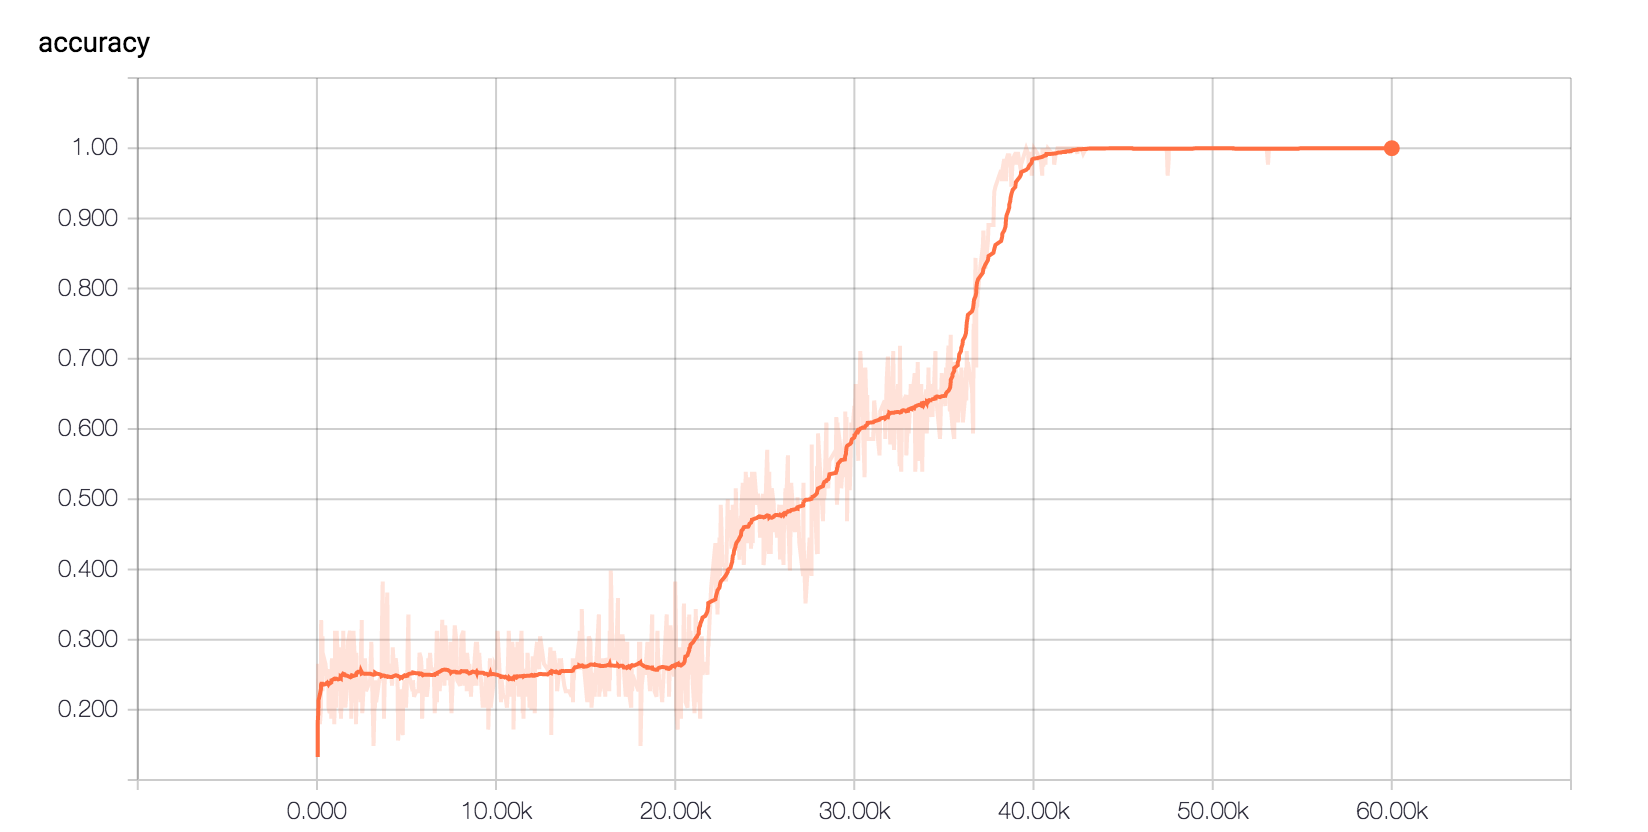
\includegraphics[scale=0.20]{../final/images/fast_weight_r_50_accuracy.png} \\
  \caption{Accuracy for the fast weights augented RNN with R=50.}
\end{figure}
